\documentclass[14pt]{extbook}
\usepackage{multicol, enumerate, enumitem, hyperref, color, soul, setspace, parskip, fancyhdr} %General Packages
\usepackage{amssymb, amsthm, amsmath, bbm, latexsym, units, mathtools} %Math Packages
\everymath{\displaystyle} %All math in Display Style
% Packages with additional options
\usepackage[headsep=0.5cm,headheight=12pt, left=1 in,right= 1 in,top= 1 in,bottom= 1 in]{geometry}
\usepackage[usenames,dvipsnames]{xcolor}
\usepackage{dashrule}  % Package to use the command below to create lines between items
\newcommand{\litem}[1]{\item#1\hspace*{-1cm}\rule{\textwidth}{0.4pt}}
\pagestyle{fancy}
\lhead{Makeup Progress Quiz 1}
\chead{}
\rhead{Version C}
\lfoot{6018-3080}
\cfoot{}
\rfoot{Spring 2021}
\begin{document}

\begin{enumerate}
\litem{
Determine the domain of the function below.\[ f(x) = \frac{5}{18x^{2} +21 x -30} \]\begin{enumerate}[label=\Alph*.]
\item \( \text{All Real numbers except } x = a, \text{ where } a \in [-21, -14] \)
\item \( \text{All Real numbers except } x = a, \text{ where } a \in [-3, -1] \)
\item \( \text{All Real numbers except } x = a \text{ and } x = b, \text{ where } a \in [-3, -1] \text{ and } b \in [0.83, 2.83] \)
\item \( \text{All Real numbers except } x = a \text{ and } x = b, \text{ where } a \in [-21, -14] \text{ and } b \in [30, 33] \)
\item \( \text{All Real numbers.} \)

\end{enumerate} }
\litem{
Solve the rational equation below. Then, choose the interval(s) that the solution(s) belongs to.\[ \frac{2x}{2x -4} + \frac{-7x^{2}}{14x^{2} -40 x + 24} = \frac{-5}{7x -6} \]\begin{enumerate}[label=\Alph*.]
\item \( x_1 \in [-1.9, -0.88] \text{ and } x_2 \in [1.88,2.1] \)
\item \( x_1 \in [-1.9, -0.88] \text{ and } x_2 \in [1.68,1.89] \)
\item \( \text{All solutions lead to invalid or complex values in the equation.} \)
\item \( x \in [0.92,4.95] \)
\item \( x \in [0.32,1.83] \)

\end{enumerate} }
\litem{
Choose the graph of the equation below.\[ f(x) = \frac{-1}{x - 1} + 3 \]\begin{enumerate}[label=\Alph*.]
\begin{multicols}{2}\item 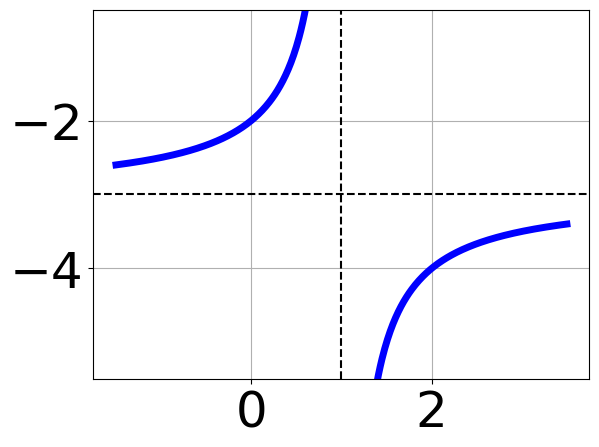
\includegraphics[width = 0.3\textwidth]{../Figures/rationalEquationToGraphCopyAC.png}\item 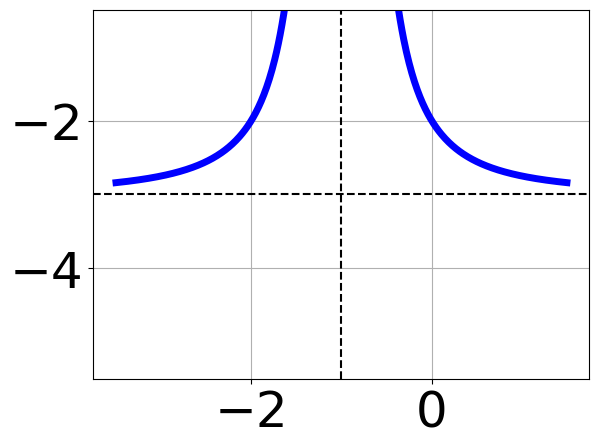
\includegraphics[width = 0.3\textwidth]{../Figures/rationalEquationToGraphCopyBC.png}\item 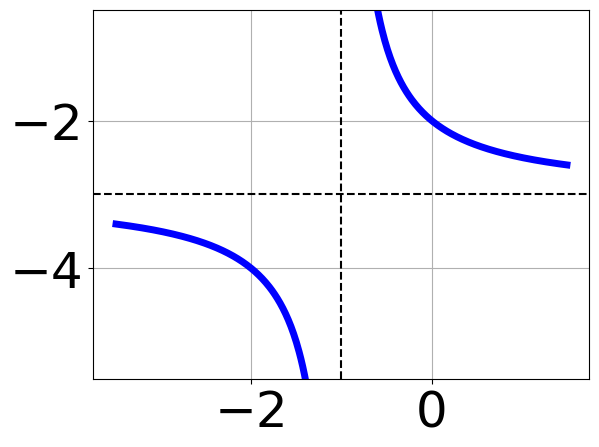
\includegraphics[width = 0.3\textwidth]{../Figures/rationalEquationToGraphCopyCC.png}\item 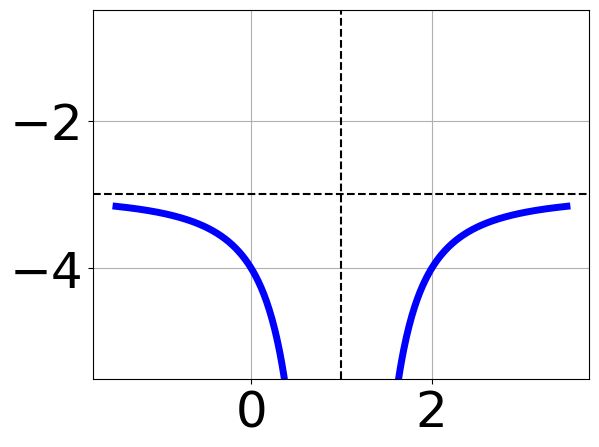
\includegraphics[width = 0.3\textwidth]{../Figures/rationalEquationToGraphCopyDC.png}\end{multicols}\item None of the above.
\end{enumerate} }
\litem{
Choose the graph of the equation below.\[ f(x) = \frac{1}{x + 1} - 1 \]\begin{enumerate}[label=\Alph*.]
\begin{multicols}{2}\item 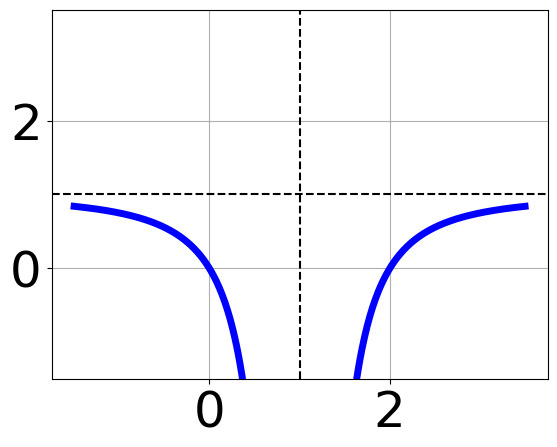
\includegraphics[width = 0.3\textwidth]{../Figures/rationalEquationToGraphAC.png}\item 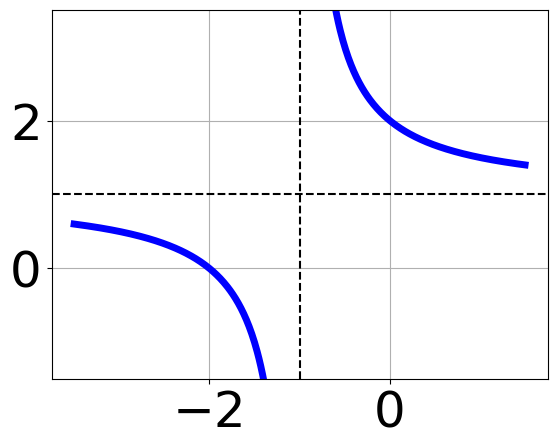
\includegraphics[width = 0.3\textwidth]{../Figures/rationalEquationToGraphBC.png}\item 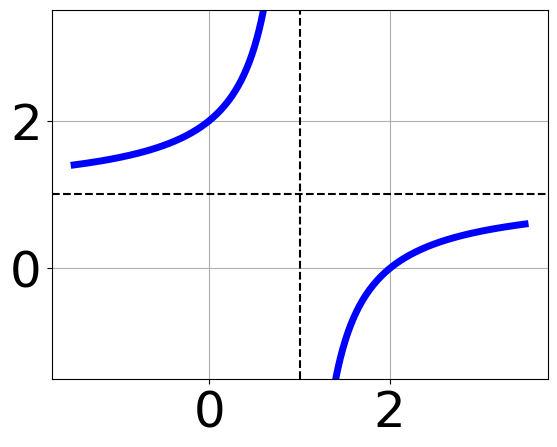
\includegraphics[width = 0.3\textwidth]{../Figures/rationalEquationToGraphCC.png}\item 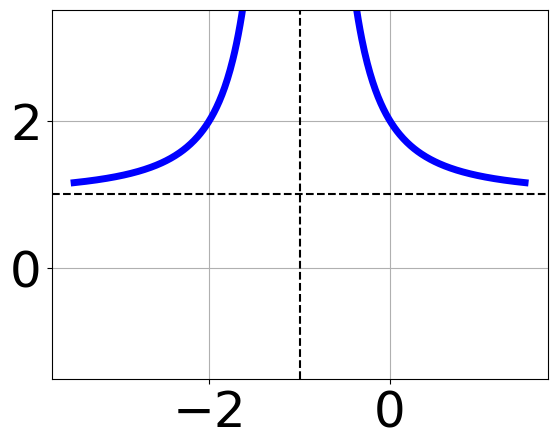
\includegraphics[width = 0.3\textwidth]{../Figures/rationalEquationToGraphDC.png}\end{multicols}\item None of the above.
\end{enumerate} }
\litem{
Choose the equation of the function graphed below.
\begin{center}
    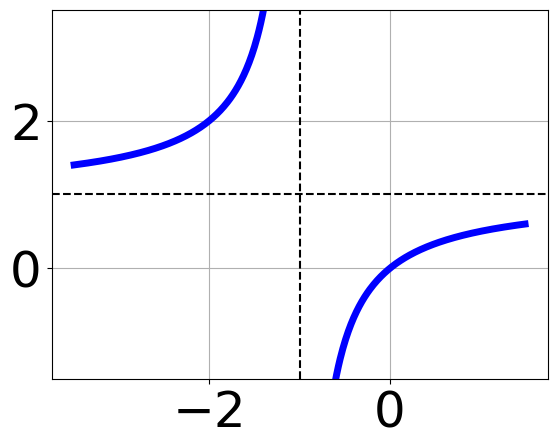
\includegraphics[width=0.5\textwidth]{../Figures/rationalGraphToEquationCopyC.png}
\end{center}
\begin{enumerate}[label=\Alph*.]
\item \( f(x) = \frac{-1}{x - 1} + 1 \)
\item \( f(x) = \frac{1}{(x + 1)^2} + 1 \)
\item \( f(x) = \frac{-1}{(x - 1)^2} + 1 \)
\item \( f(x) = \frac{1}{x + 1} + 1 \)
\item \( \text{None of the above} \)

\end{enumerate} }
\litem{
Solve the rational equation below. Then, choose the interval(s) that the solution(s) belongs to.\[ \frac{-3x}{-2x -4} + \frac{-4x^{2}}{4x^{2} +22 x + 28} = \frac{6}{-2x -7} \]\begin{enumerate}[label=\Alph*.]
\item \( x_1 \in [-16.05, -15.64] \text{ and } x_2 \in [-2.8,-1.3] \)
\item \( \text{All solutions lead to invalid or complex values in the equation.} \)
\item \( x_1 \in [-16.05, -15.64] \text{ and } x_2 \in [-1.4,-0.3] \)
\item \( x \in [-2.18,1.01] \)
\item \( x \in [-4.57,-3.01] \)

\end{enumerate} }
\litem{
Determine the domain of the function below.\[ f(x) = \frac{6}{30x^{2} -2 x -12} \]\begin{enumerate}[label=\Alph*.]
\item \( \text{All Real numbers.} \)
\item \( \text{All Real numbers except } x = a \text{ and } x = b, \text{ where } a \in [-0.6, 0.4] \text{ and } b \in [-0.33, 1.67] \)
\item \( \text{All Real numbers except } x = a, \text{ where } a \in [-19, -12] \)
\item \( \text{All Real numbers except } x = a \text{ and } x = b, \text{ where } a \in [-19, -12] \text{ and } b \in [23, 28] \)
\item \( \text{All Real numbers except } x = a, \text{ where } a \in [-0.6, 0.4] \)

\end{enumerate} }
\litem{
Choose the equation of the function graphed below.
\begin{center}
    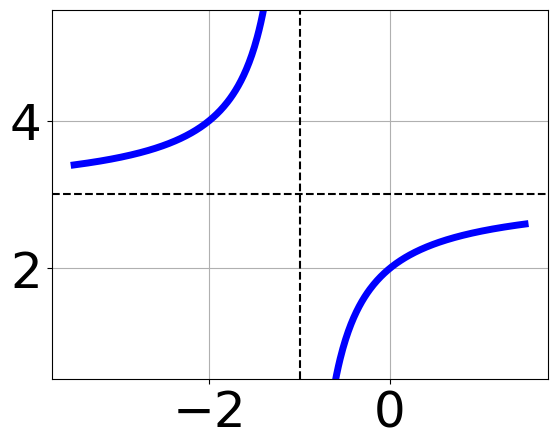
\includegraphics[width=0.5\textwidth]{../Figures/rationalGraphToEquationC.png}
\end{center}
\begin{enumerate}[label=\Alph*.]
\item \( f(x) = \frac{1}{x - 1} + 3 \)
\item \( f(x) = \frac{-1}{(x + 1)^2} + 3 \)
\item \( f(x) = \frac{-1}{x + 1} + 3 \)
\item \( f(x) = \frac{1}{(x - 1)^2} + 3 \)
\item \( \text{None of the above} \)

\end{enumerate} }
\litem{
Solve the rational equation below. Then, choose the interval(s) that the solution(s) belongs to.\[ \frac{-56}{-24x + 48} + 1 = \frac{-56}{-24x + 48} \]\begin{enumerate}[label=\Alph*.]
\item \( \text{All solutions lead to invalid or complex values in the equation.} \)
\item \( x \in [1.0,4.0] \)
\item \( x_1 \in [-2, 1] \text{ and } x_2 \in [2,4] \)
\item \( x \in [-2,1] \)
\item \( x_1 \in [1, 5] \text{ and } x_2 \in [2,4] \)

\end{enumerate} }
\litem{
Solve the rational equation below. Then, choose the interval(s) that the solution(s) belongs to.\[ \frac{3}{8x -7} + 7 = \frac{-9}{-56x + 49} \]\begin{enumerate}[label=\Alph*.]
\item \( x \in [0.84,1.84] \)
\item \( x_1 \in [0.4, 0.84] \text{ and } x_2 \in [0.84,1.84] \)
\item \( x \in [-1.06,-0.59] \)
\item \( x_1 \in [-1.06, -0.59] \text{ and } x_2 \in [0.84,1.84] \)
\item \( \text{All solutions lead to invalid or complex values in the equation.} \)

\end{enumerate} }
\end{enumerate}

\end{document}